% Created 2026-07-06 Mon 21:56
\documentclass{article}
\usepackage[utf8]{inputenc}
\usepackage[T1]{fontenc}
\usepackage{graphicx}
\usepackage{longtable}
\usepackage{wrapfig}
\usepackage{rotating}
\usepackage[normalem]{ulem}
\usepackage{amsmath}
\usepackage{amssymb}
\usepackage{capt-of}
\usepackage{hyperref}

\usepackage{fancyhdr}
\usepackage[top=25mm, left=25mm, right=25mm]{geometry}
\usepackage{longtable}
\fancyhead[R]{}
\setlength\headheight{43.0pt}
\usepackage{tabularx}
\usepackage{longtable}
\usepackage[backend=biber, style=ieee]{biblatex}
\addbibresource{/home/mick/bibliography/bibliography.bib}
\author{Danilo Unapucha, Michael Sornoza , Matías Palomeque, y Sebastian Arevalo}
\date{2026-05-24}
\title{Taller - Conceptos Básicos de Hardware y Ensamblaje de Computadores\\\medskip
\large ICCD332 Arquitectura de Computadores }
\hypersetup{
 pdfauthor={Danilo Unapucha, Michael Sornoza , Matías Palomeque, y Sebastian Arevalo},
 pdftitle={Taller - Conceptos Básicos de Hardware y Ensamblaje de Computadores},
 pdfkeywords={},
 pdfsubject={},
 pdfcreator={Emacs 29.3 (Org mode 9.6.15)}, 
 pdflang={Spanish}}
\begin{document}

\maketitle
\fancyhead[C]{\includegraphics[scale=0.05]{../images/logoEPN.jpg}\\
ESCUELA POLITECNICA NACIONAL\\FACULTAD DE INGENIERIA DE SISTEMAS\\
ARQUITECTURA DE COMPUTADORES}
\thispagestyle{fancy}


\section{Instrucciones generales}
\label{sec:orgf2efcaa}

Este taller se realiza en \textbf{grupos}. Cada integrante debe completar
individualmente el curso Cisco Networking Academy:
\textbf{Conceptos Básicos de Hardware de Computadora} y obtener su
certificado de completitud. 

\textbf{Entregables del grupo:}
\begin{itemize}
\item Resolución de éste archivo fuente \texttt{.org}
\item El PDF exportado desde Emacs \texttt{M-x org-latex-export-to-pdf}
\item Los certificados individuales de cada integrante (PDF o imagen)
\end{itemize}


\textbf{Entregable Individual(Tarea):}
\begin{itemize}
\item Resolver el cuestionario individual en el aula virtual
\end{itemize}
\subsection{Recursos}
\label{sec:org882acd8}
Cree su usuario en la plataforma de \emph{Cisco Networking Academy}. Use el
siguiente enlace:

\href{https://www.netacad.com/es/courses/computer-hardware-basics?courseLang=en-US}{Cisco Computer Hardware Basics}

Puede configurar según el idioma de su preferencia. El texto está
disponible en Español. Los vídeos disponen de subtítulos en varios
idiomas.

\section{Parte A. Integrantes y certificados\hfill{}\textsc{x}}
\label{sec:org97fa218}
Para insertar la captura del certificado utilice YASnippet: Escriba
\texttt{fig\_} seguido de \texttt{C-TAB}. Esto produce \texttt{\#+caption}, \texttt{\#+attr\_latex} y
\texttt{\#+label} que permiten colocar un encabezado a la imagen, controlar el
escalado de la misma y una referencia. Finalmente inserte el enlace al
archivo usando \texttt{C-c C-l} o usando \texttt{[[./carpeta-certificados/cert-int1.pdf]]}
\begin{enumerate}
\item \textbf{Integrante 1}
\begin{itemize}
\item \textbf{Nombre completo:} Danilo Unapucha
\item \textbf{Correo:} danilo.unapucha@epn.edu.ec
\item \textbf{Certificado adjunto:}
\end{itemize}
\end{enumerate}

\begin{figure}[htbp]
\centering
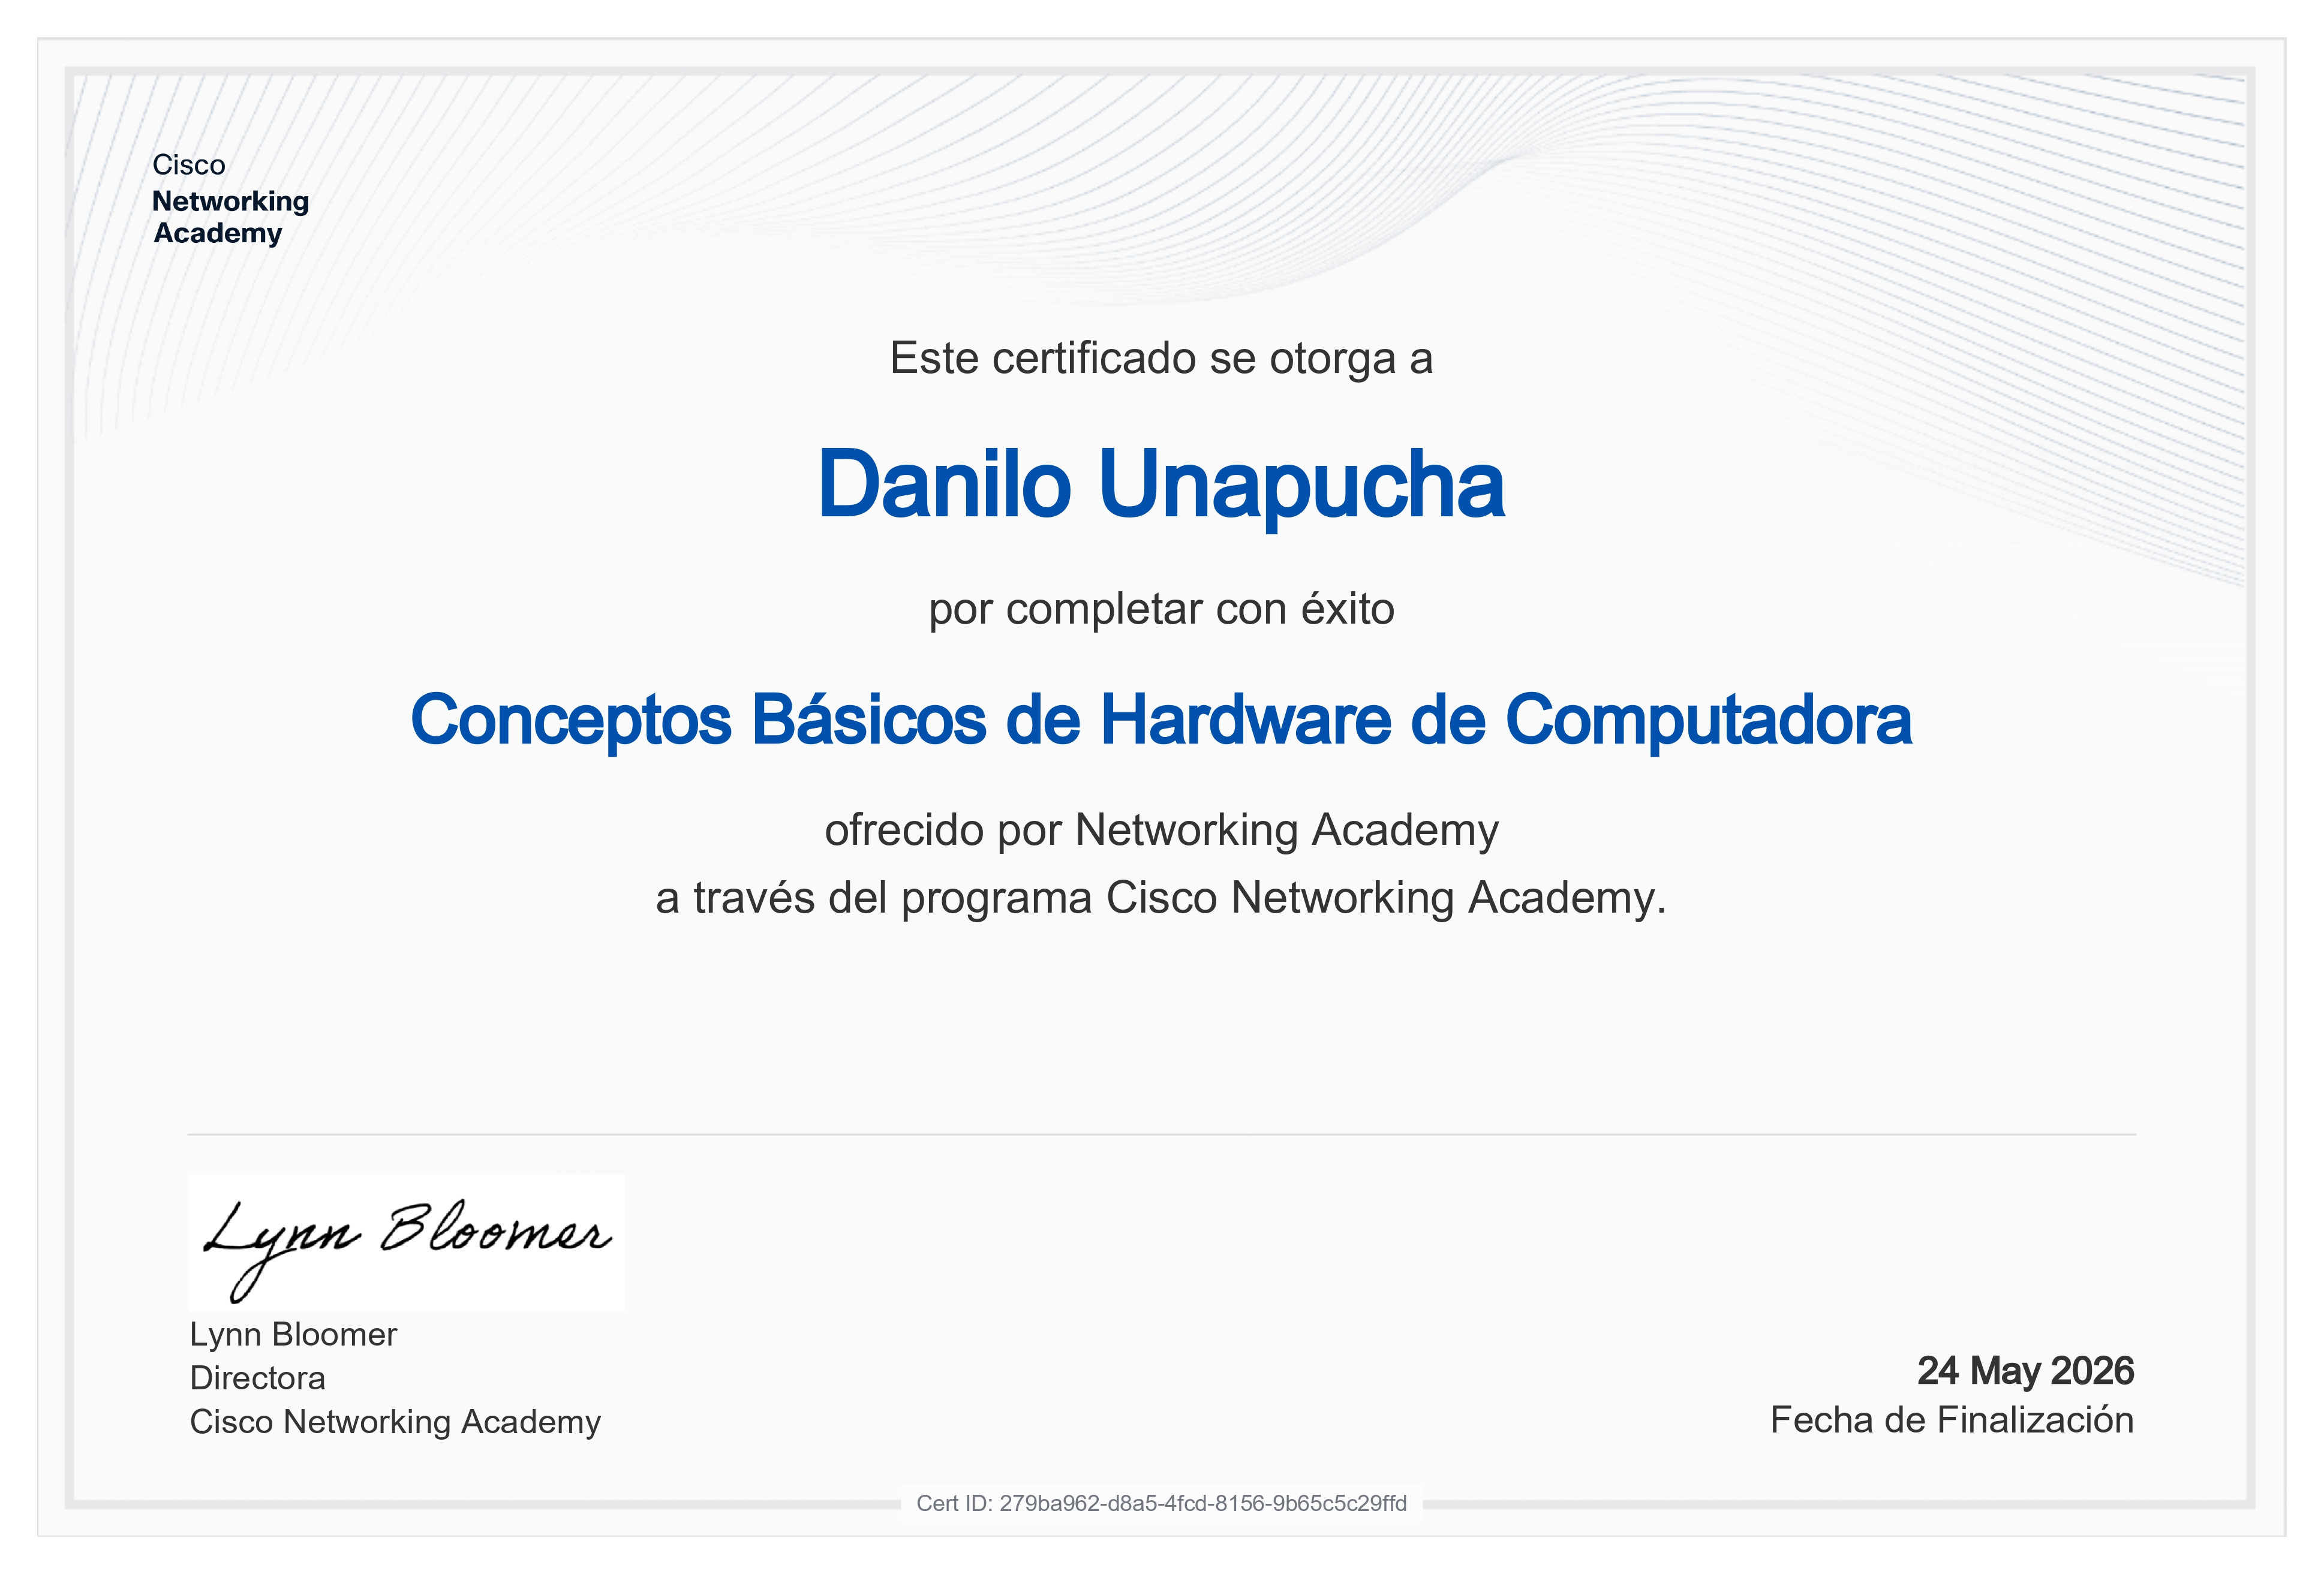
\includegraphics[width=0.75\textwidth]{./images/Danilo_Certificado.jpg}
\caption{\label{fig:orgb262188}Certificado de Aprobación - Danilo Unapucha}
\end{figure}

\begin{enumerate}
\item Integrante 2
\begin{itemize}
\item Nombre completo: Michael Sornoza
\item Correo: michael.sornoza@epn.edu.ec
\item Certificado adjunto:
\end{itemize}
\end{enumerate}

\begin{figure}[htbp]
\centering
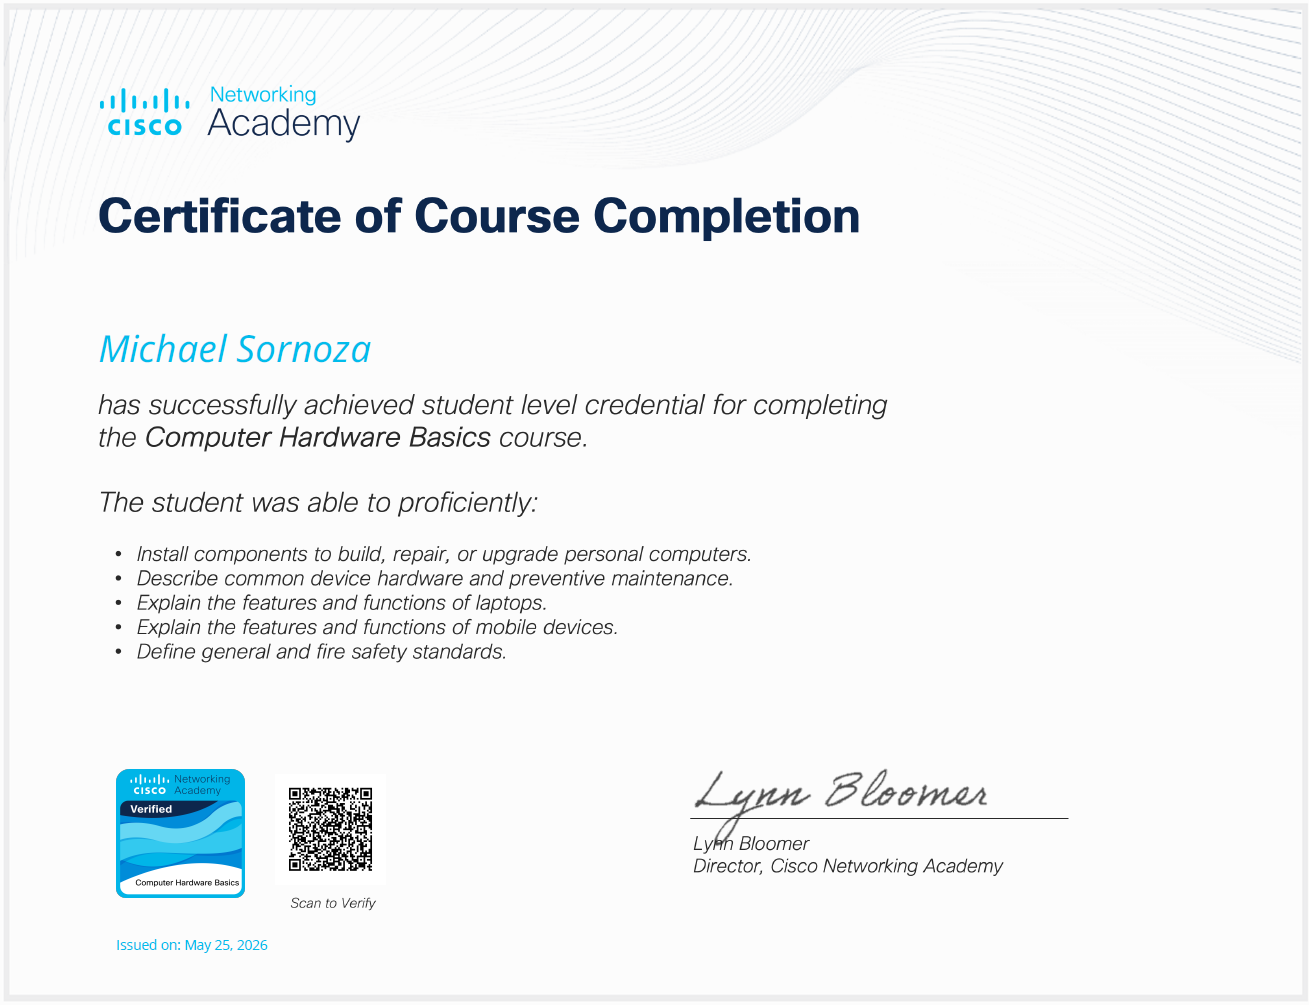
\includegraphics[width=0.75\textwidth]{./images/Certificado_Michael.png}
\caption{\label{fig:org4c1163c}Certificado de Aprobación - Michael Sornoza}
\end{figure}

\begin{enumerate}
\item \textbf{Integrante 3}
\begin{itemize}
\item \textbf{Nombre completo:} Matías Palomeque
\item \textbf{Correo:} matias.palomeque@epn.edu.ec
\item \textbf{Certificado Adjunto}
\end{itemize}
\end{enumerate}

\begin{figure}[htbp]
\centering
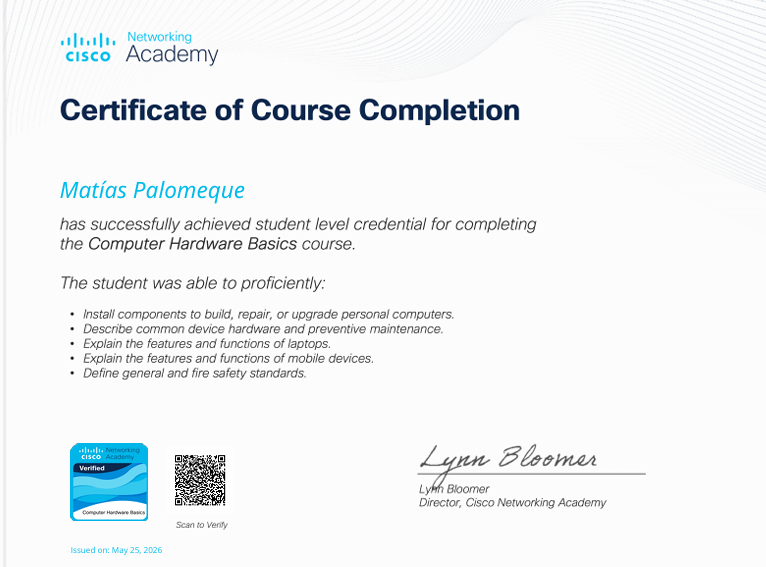
\includegraphics[width=0.75\textwidth]{./images/CertificadoMatias.png}
\caption{\label{fig:org1207ae2}Certificado de Aprobación - Matías Palomeque}
\end{figure}


\begin{enumerate}
\item \textbf{Integrante 4}
\begin{itemize}
\item \textbf{Nombre completo:} Sebastian Arevalo
\item \textbf{Correo:} martin.arevalo@epn.edu.ec
\item \textbf{Certificado Adjunto}
\end{itemize}
\end{enumerate}

\begin{figure}[htbp]
\centering
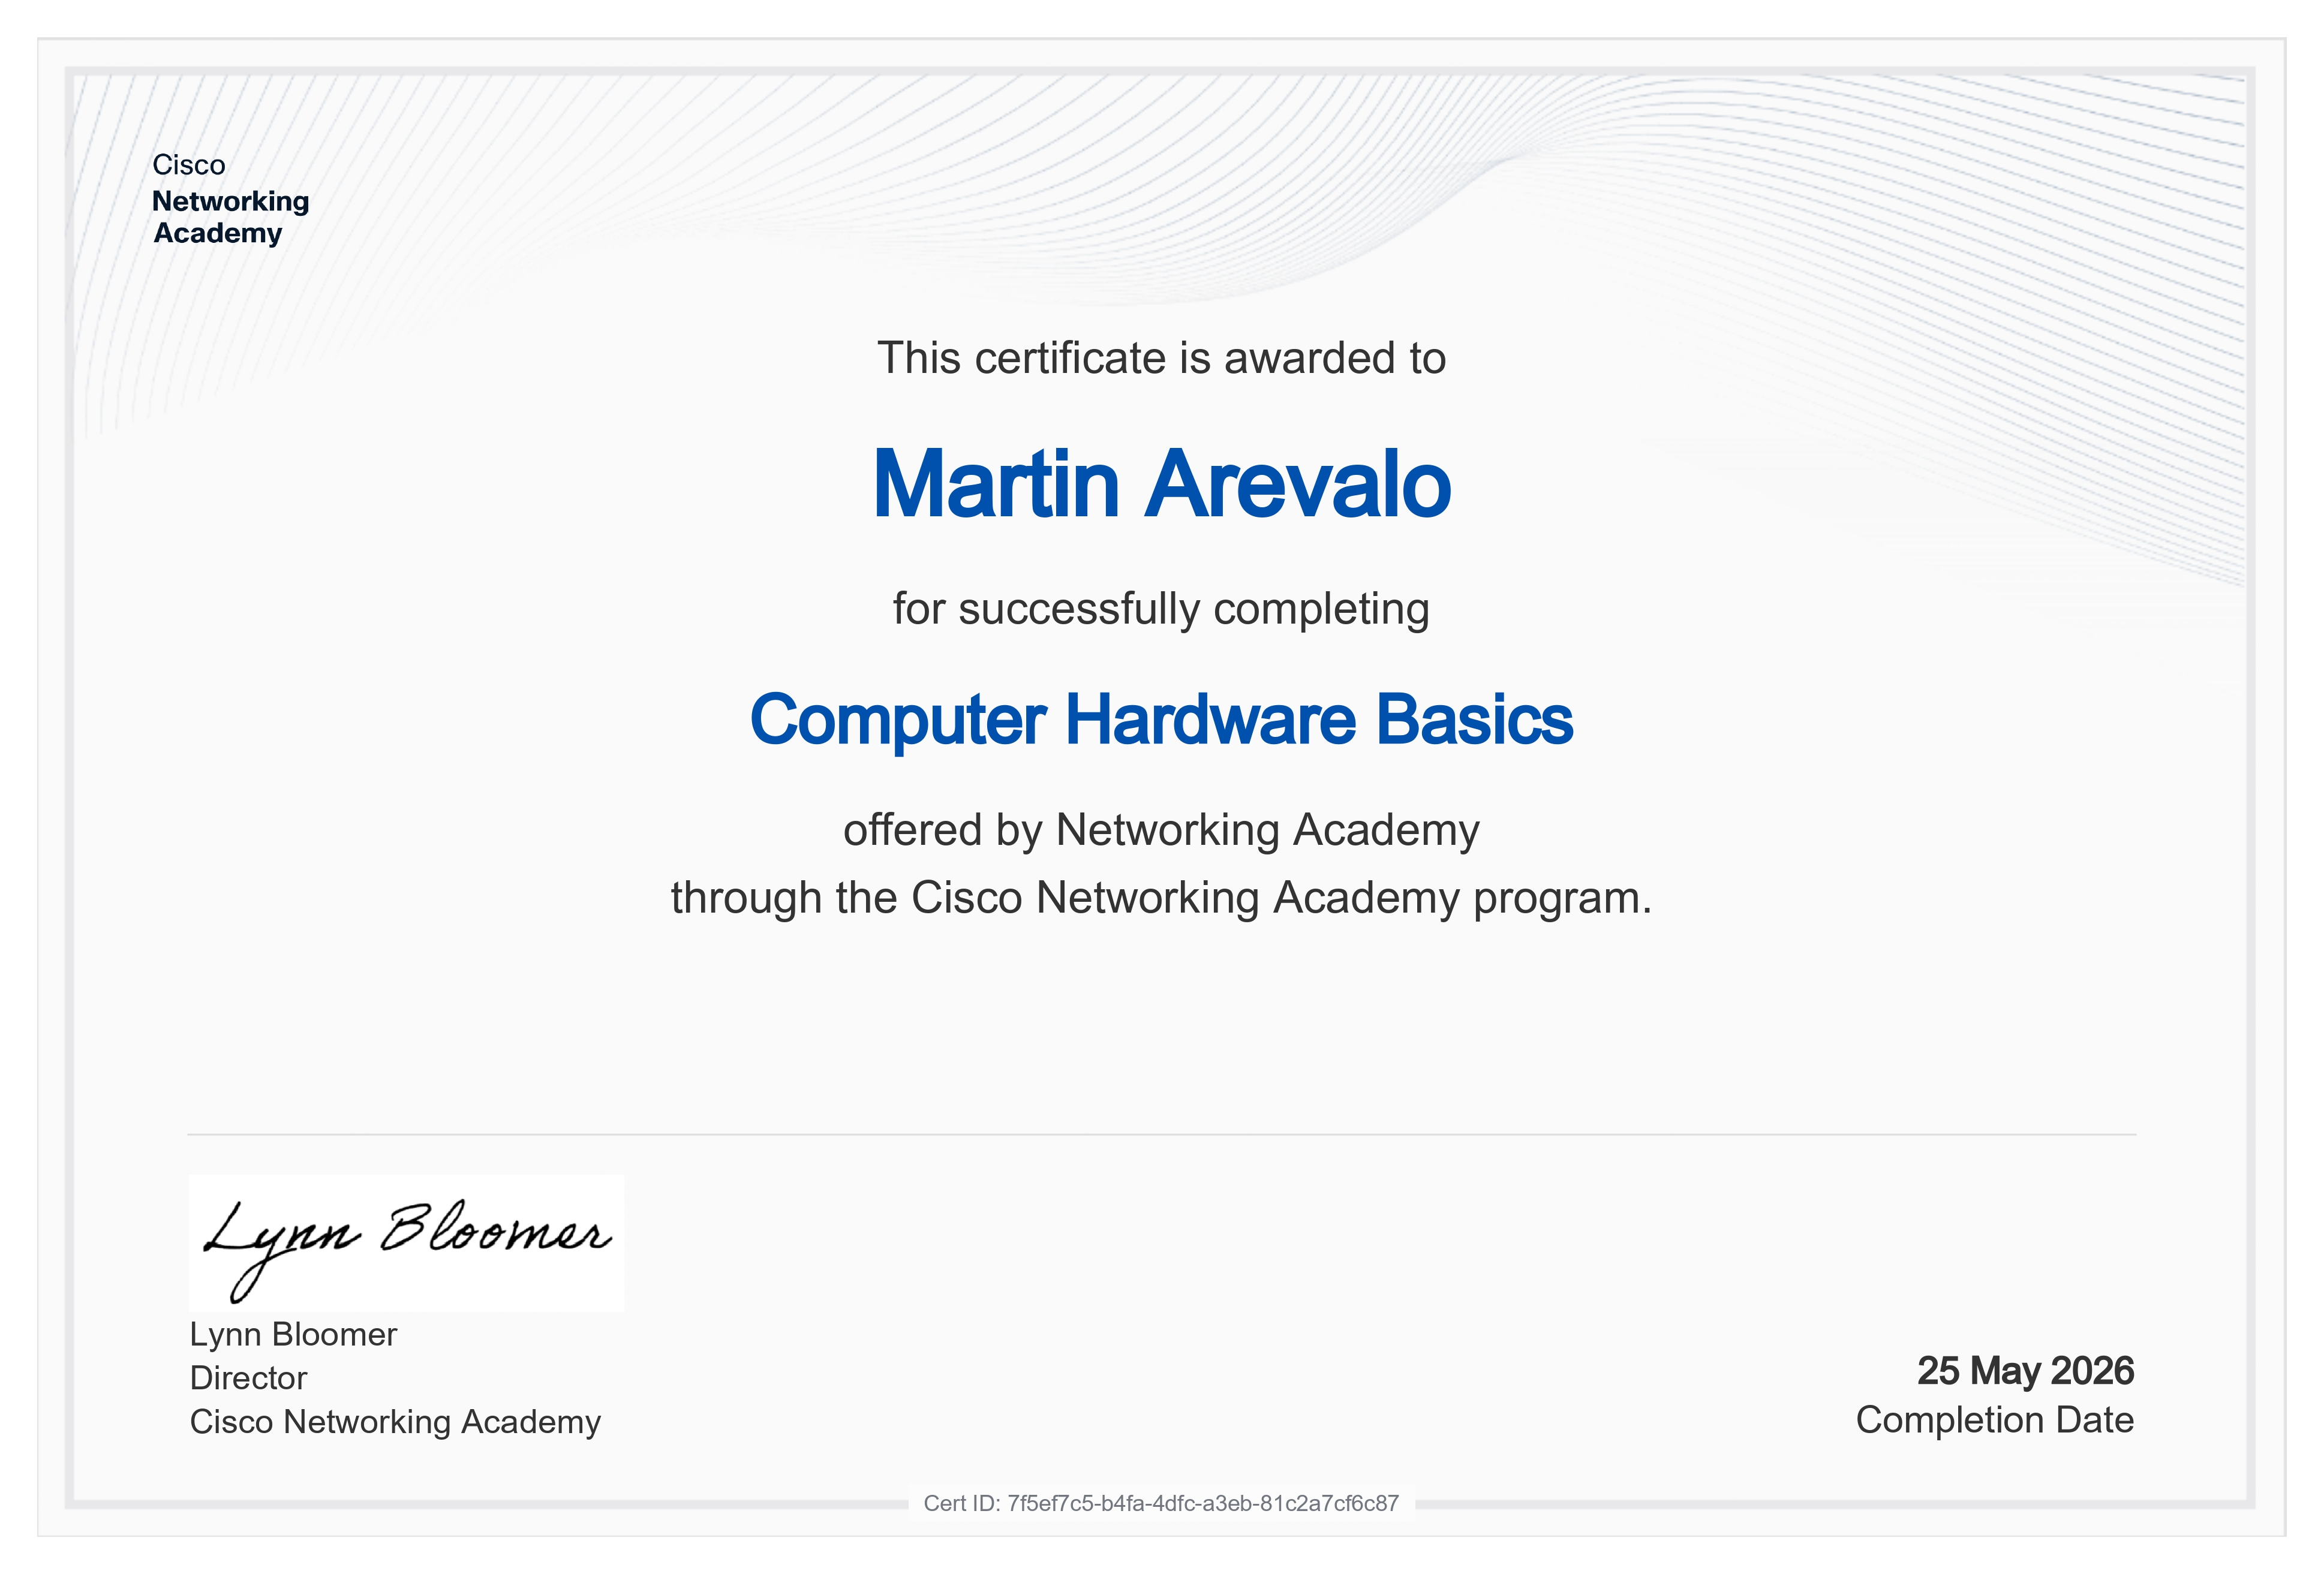
\includegraphics[width=0.75\textwidth]{./images/Sebas_certificado.jpg}
\caption{\label{fig:org2449c7e}Certificado de Aprobación - Sebastian Arevalo}
\end{figure}

\section{Parte B. Cuestionario argumentado grupal}
\label{sec:orgf57d96b}

Para cada pregunta:

\begin{itemize}
\item Indique la alternativa escogida (letra).
\item Escriba una justificación técnica breve (3 a 6 líneas). Fundamente
su respuesta. Su insumo principal es el curso de Conceptos Básicos
de Hardware. Si usa otro material referenciar.
\item Discuta con el grupo de trabajo las opciones y la respuesta ¿Existió
consenso? ¿Cuáles fueron las principales discrepancias?
\end{itemize}

\textbf{Criterio:} correcto/incorrecto + calidad del argumento técnico.

\subsection{Pregunta 1}
\label{sec:org9e5a47c}
Al instalar una CPU en un socket LGA, ¿por qué es crítico alinear el
pin 1 de la CPU con el pin 1 del socket?

a. Para que el sistema arranque con mayor rapidez 

b. Para evitar daños en la CPU y el socket al insertar incorrectamente

c. Porque el pin 1 es el único que conduce electricidad 

d. Para que el disipador quede centrado automáticamente

Estudiante: Danilo Unapucha

\begin{itemize}
\item \emph{Alternativa escogida:} b
\item \emph{Justificación técnica:} Esto se debe a que le socket tiene pines
muy delicados y si no se ponen correctamente pueden llegar a
romperse
\end{itemize}

Estudiante: Michael Sornoza 

\begin{itemize}
\item \emph{Alternativa escogida:} b
\item \emph{Justificación técnica:} El poner mal el orden de los pines ocasionaría que se dañen
los componentes electeónicos, porque cada pin lleva electricidad a un componente
diferente y se se le da un mal voltaje a un componente se puede dañar el componente
y en el peor de los casos varios circuitos.
\end{itemize}

Estudiante: Matías Palomeque

\begin{itemize}
\item \emph{Alternativa escogida:} b
\item \emph{Justificación técnica:} Los pines tienen un orden específico, ya
que garantizan que cada componente reciba la cantidad de corriente
y/o voltaje necesaria. Ingresarlos en otro orden del establecido
podría generar cortocircuitos.

Estudiante: Sebastian Arevalo

\item \emph{Alternativa escogida:} b
\end{itemize}
-\emph{Justificación técnica:} Sis e colocan los pines en un orden
incorrecto la carga de corriete que resivira cada uno sera distinta a
la que estan diseñados para resistir o funcionar probocando daños que
pueden ser permanentes. 

\begin{itemize}
\item \emph{Debate del grupo:} [a completar]
\end{itemize}


\subsection{Pregunta 2}
\label{sec:orgeb4adcc}
Al montar la placa madre en el gabinete, ¿cuál es la función de los separadores (standoffs)?

a. Sostener el peso de las tarjetas de expansión

b. Evitar cortocircuitos entre la placa madre y el metal del gabinete

c. Mejorar la ventilación de la placa madre

d. Facilitar la alineación del panel de E/S trasero

Estudiante: Danilo Unapucha

\begin{itemize}
\item \emph{Alternativa escogida:} b
\item \emph{Justificación técnica:} Estos tienen como función que la placa
madre no toque con la tapa metálica de atrás para que los circuitos
no toquen y no hagan cortocircuito
\end{itemize}

Estudiante: Michael Sornoza

\begin{itemize}
\item \emph{Alternativa escogida:} b
\item \emph{Justificación técnica:} De esta manera se protege los componentes del metal, esto se debe que en
la placa hay varios circuitos con componentes y soldadura que conducen electricidad y al tener contacto
con el metal ocasionaría un cortocircuito.
\end{itemize}

Estudiante: Matías Palomeque

\begin{itemize}
\item \emph{Alternativa escogida:} b
\item \emph{Justificación técnica:} Los separadores evitan el contacto  entre
la placa madre y el metal del gabinete, ya que el metal puede
conducir electricidad. Esto podría ocasionar que exista un
cortocircuito en la placa madre y la dañe completamente.
\end{itemize}

Estudiante: Sebastian Arevalo

\begin{itemize}
\item \emph{Alternativa escogida:} b
\item \emph{Justificación técnica:} Al separar la placa madre del gabinete se
evitan problemas con el contacto de los circuitos con el metal del
gabinete de ya que el contacto podria probocar daños por una mala
transferencia de electricidad.

\item \emph{Debate del grupo:} [a completar]
\end{itemize}


\subsection{Pregunta 3}
\label{sec:orgf8a445a}
Según el manual de ensamblaje de Cisco, ¿cuándo NO es necesario aplicar pasta térmica al instalar el disipador sobre la CPU?

a. Cuando la CPU es de alto rendimiento

b. Cuando el disipador ya incluye pasta térmica preaplicada

c. Cuando la CPU tiene más de un año de uso

d. Cuando el gabinete tiene buena ventilación

Estudiante: Danilo Unapucha

\begin{itemize}
\item \emph{Alternativa escogida:} b
\item \emph{Justificación técnica:} En la actualidad ya la mayoría de
disipadores ya vienen así y no hace falta poner mas pasta térmica sino seria un desperdicio
\end{itemize}

Estudiante: Michael Sornoza

\begin{itemize}
\item \emph{Alternativa escogida:} b
\item \emph{Justificación técnica:} La pasta térmica es escencial en un equipo porque ayuda a distribuir el calor
el único escenario en el que no se le aplica es cuando el dispostivo es nuevo y ya tiene aplicada
de fábrica la pasta, caso contrario siempre en un mantenimiento hay que aplicar la pasta térmica.
\end{itemize}

Estudiante: Matías Palomeque

\begin{itemize}
\item \emph{Alternativa escogida:} b
\item \emph{Justificación técnica:} La pasta térmica ayuda a distrubuir
correctamente el calor y evita que los componentes se
sobrecalienten. Es necesario colocarla siempre, excepto cuando el
disipador ya tiene pasta térmica aplicada, ya que el exceso de pasta
podría hacer que haya errores en la aplicación y podrían existir problemas.
\end{itemize}

Estudiante: Sebastian Arevalo

\begin{itemize}
\item \emph{Alternativa escogida:} b
\item \emph{Justificación técnica:} Si el sistema de dispercion de de calor de
la computadora ya tine pre puesta pasta termica ya no es necesario
poner mas hasta que la misma ya no este en condiciones.

\item \emph{Debate del grupo:} [a completar]
\end{itemize}


\subsection{Pregunta 4}
\label{sec:orgf47de32}
¿Por qué se recomienda usar pulsera antiestática y alfombrilla antiestática al manipular componentes internos?

a. Para proteger al técnico de descargas de 220 V

b. Para evitar que la electricidad estática dañe los componentes

c. Para cumplir una norma estética del laboratorio

d. Para que los tornillos no se magneticen

Estudiante: Danilo Unapucha

\begin{itemize}
\item \emph{Alternativa escogida:} b
\item \emph{Justificación técnica:} Porque nuestro cuerpo acumula la
electricidad estática y esta si se aplica a un componente de la pc
es suficiente para quemarlo esto es lo que evita la pulsera y la
alfombrilla mandado esta electricidad a tierra
\end{itemize}

Estudiante: Michael Sornoza

\begin{itemize}
\item \emph{Alternativa escogida:} b
\item \emph{Justificación técnica:} La electricidad estática es un problema muy común y que involuntariamente las personas
sabemos producirlas y al transferir esa electricidad a los componenetes electrónicos más delicados pueden
dañarse, por eso la pulsera y la alfombra redirigen a tierra.
\end{itemize}

Estudiante: Matías Palomeque

\begin{itemize}
\item /Alternativa escogida: b
\item \emph{Justificación técnica:} Nuestro cuerpo tiende a acumular
electricidad estática al solo frotar cosas que conducen la
electricidad. Si bien no es mucho voltaje, los componentes de la PC
son sumamente frágiles, y pueden dañarse con voltajes tan pequeños
como 20V. Una pulsera antiestática ayuda a evitar que conduzcamos
electricidad estática y así poder manejar componentes delicados sin
peligro de dañarlos.
\end{itemize}

Estudiante: Sebastian Arevalo

\begin{itemize}
\item /Alternativa escogida: b
\item \emph{Justificación técnica:} El cuerpo humano acumula electricidad
estatica de manera que esta si no se usa equipo anti estatico puede
llegar a los componentes que pueden sufrir daños permanentes al no
agunatar la electricidad que les llega.
\end{itemize}


\begin{itemize}
\item \emph{Debate del grupo:} [a completar]
\end{itemize}


\subsection{Pregunta 5}
\label{sec:org9e45a7b}
Si al iniciar la computadora por primera vez un LED del panel frontal no funciona, ¿qué indica el manual de Cisco?

a. Reemplazar el conector por uno de repuesto

b. Revisar el BIOS para habilitar el LED

c. Quitar el conector, invertirlo y volver a conectarlo

d. Desconectar y reconectar la fuente de poder

Estudiante: Danilo Unapucha

\begin{itemize}
\item \emph{Alternativa escogida:} c
\item \emph{Justificación técnica:} Esto seria un buen primer paso ya que por
lo general se conectan mal estos conectores al tener polaridad ya si
después de esto sigue el mismo problema seria de preocuparse
\end{itemize}

Estudiante: Michael Sornoza

\begin{itemize}
\item \emph{Alternativa escogida:} c
\item \emph{Justificación técnica:} Probablemente el LED no fue conectado correctamente y si bien es una mala
práctica  invertirlos resolvería el problema, lo ideal es ver el manual donde este el esquema para conectar bien los LED
en el curso mostraba un esquema que podiamos seguir para no tener errores.
\end{itemize}

Estudiante: Matías Palomeque

\begin{itemize}
\item \emph{Alternativa escogida:} c
\item \emph{Justificación técnica:} El LED del panel frontal en una PC tiene
polaridad, por lo que si no funciona, lo más probable es que esté
conectado en sentido contrario. Es por esto, que es recomendable
invertir las conexiones y volver a probar.
\end{itemize}

Estudiante: Sebastian Arevalo

\begin{itemize}
\item \emph{Alternativa escogida:} c
\item \emph{Justificación técnica:} Cuando un led no prende lo mas probable es
que este conectado de manera invertida asi que el probar conectarlo
invirtiendo la polaridad podria arreglar el problema.
\end{itemize}


\begin{itemize}
\item \emph{Debate del grupo:} [a completar]
\end{itemize}

\subsection{Pregunta 6}
\label{sec:orga7f650c}
¿Por qué una GPU puede requerir un conector de alimentación PCIe adicional de la fuente de poder?

a. Porque la ranura PCIe no transmite señal de video

b. Porque las GPUs de alto rendimiento consumen más potencia de la que la ranura puede suministrar

c. Porque el conector PCIe solo funciona con tarjetas de red

d. Por el estándar de codificación de color de los cables SATA

Estudiante: Danilo Unapucha

\begin{itemize}
\item \emph{Alternativa escogida:} b
\item \emph{Justificación técnica:} Porque si solo se le suministra la energía
que viene del conector no es suficiente y la placa se sobre cargara
por eso se conecta directo a la fuente esto claro en GPUs de mas
alta gama
\end{itemize}

Estudiante: Michael Sornoza

\begin{itemize}
\item \emph{Alternativa escogida:} b
\item \emph{Justificación técnica:} Las tarjetas gráficas actuales usualmente necesitan más energía de las que
da la ranura por eso se las conecta directo a la fuente de alimentación, además es un dato muy importante
escoger una buena fuente para que de la suficiente energia a todos los componentes que saben consumir
mucha energia por sus características como la GPU.
\end{itemize}

Estudiante: Matías Palomeque

\begin{itemize}
\item \emph{Alternativa escogida:} b
\item \emph{Justificación técnica:} La ranura PCIe de la placa madre puede
suministrar una cantidad de energía limitada, pero las tarjetas
gráficas más actuales utilizan más potencia de la que pueden
suministrar. Es por esto que pueden requerir un conector extra, así
puede funcionar correctamente y cumplir todas sus funciones
\end{itemize}

Estudiante: Sebastian Arevalo

\begin{itemize}
\item \emph{Alternativa escogida:} b
\item \emph{Justificación técnica:} LAs tarjetas graficas pueden consumir
cantidades muy grnades de energia haciendo que la que la energia
suministrada quede corta necesitando una coneccion extra

\item \emph{Debate del grupo:} [a completar]
\end{itemize}

\section{Parte C. Mantenimiento de computadores}
\label{sec:org703f9ba}

\subsection{3.1 Insumos para mantenimiento preventivo}
\label{sec:orgbccee02}
Liste al menos seis insumos y describa para qué sirve cada
uno. Revise el siguiente \href{https://youtu.be/3ri1BMV7XTM?si=bjYoDUUKuMWwj4Qg}{vídeo}.

Estudiante: Danilo Unapucha

\begin{center}
\begin{tabular}{ll}
Insumo & Uso principal\\[0pt]
\hline
Aire comprimido & Elimina el polvo en ventiladores\\[0pt]
Pasta Térmica & Enfrían los componentes que generan calor\\[0pt]
Destornilladores & Abren el gabinete y sueltan al procesador\\[0pt]
Alcohol Isopropilico & Limpia contactos y resto de pasta térmica\\[0pt]
Brocha Antiestática & Remueve el polvo de zonas de la placa madre\\[0pt]
Paño Micro fibra & Limpieza carcasas sin dejar pelusas\\[0pt]
\end{tabular}
\end{center}

Estudiante: Michael Sornoza

\begin{center}
\begin{tabular}{ll}
Insumo & Uso principal\\[0pt]
\hline
Compartmientos y etiquetas & Cuando se quita los tornillos y piezas es recomendado clasificarlos y nombrarlos\\[0pt]
Espuma limpiadora & Se aplica con un cepillo en los coolers para remover suciedad entre aspas\\[0pt]
Cinta resistente al calor & Se coloca entre los ventiladores y las alteas del disipador (aprovecha todo el fluje de aire)\\[0pt]
Thermal Putty & Se aplica sobre las memorias VRAM y sobre la VRM\\[0pt]
Aspiradora & Es una buena alternativa para extrer toda la suciedad en la carcasa\\[0pt]
Alchol isopropilico & Ayuda a limpirar la pasta sobrante, y suciedad alojada en componentes\\[0pt]
\end{tabular}
\end{center}

Estudiante: Matías Palomeque

\begin{center}
\begin{tabular}{ll}
Insumo & Uso principal\\[0pt]
\hline
Pulsera antiestática & Evita que se acumule electricidad estática en el cuerpo\\[0pt]
Aire Comprimido & Elimina el polvo entre los componentes de manera segura\\[0pt]
Destornillador con punta Metálica & Se usa para abrir compartimientos cerrados con tornillos, la punta ayuda a sostenerlos\\[0pt]
Pasta Térmica & Ayuda a distribuir el calor en los componentes de mejor manera\\[0pt]
Pinzas de Precisión & Se usan para poder sujetar componentes pequeños\\[0pt]
Espuma Limpiadora & Se utiliza para poder limpiar la suciedad entre las aspas de los ventiladores\\[0pt]
 & \\[0pt]
\end{tabular}
\end{center}

Estudiante: Sebastian Arevalo

\begin{center}
\begin{tabular}{ll}
Insumo & Uso principal\\[0pt]
\hline
Pasta termica & Ayuda a distribuir el calor desde el CPU hacia el disipador\\[0pt]
Cinta resistente al calor & Ayuda a sostener siertas partes como el sistema de refrigeracion ya que resiste altas temperaturas\\[0pt]
Alcohol isopropilico & Con este se puede limpiar de manera profunda dispositivos electronicos sin dañar los circuitos\\[0pt]
Aire comprimido & Permite limpiar los ventiladores y partes dificiles de alcanzar llenas de polvo\\[0pt]
Destornillador con punta metalica & Importante para abrir el dispostivo con facilidad y no perder los tornillos en el proseso\\[0pt]
THermal Putty & Grasa que ayuda con la disipacion del calor\\[0pt]
\end{tabular}
\end{center}

\subsection{3.2 Procedimiento de limpieza — Desktop}
\label{sec:org309f34c}
\begin{enumerate}
\item Apagar completamente la computadora y desconectarla de corriente eléctrica
\item Desconectar la fuente de poder y retirar los cables necesarios
\item Desconectar los ventiladores y demás componentes que eviten el
facil acceso al interior de la PC
\item Realizar la limpieza del polvo acumulado en los componentes,
especialmente de los ventiladores y la placa madre. Para esto es
recomendable utilizar aire comprimido
\item Limpiar la superficie de la CPU y GPU con alcohol isopropílico
para retirar restos de pasta térmica antigua. Luego, aplicar
nueva pasta térmica y reemplazar los pads térmicos de ser
necesario.
\item Utilizar una brocha antiestática para realizar una limpieza final
antes de reensamblar los componentes
\item Reconectar todos los componentes y verificar que las conexiones
estén correctamente instaladas antes de volver a enceder la computadora
\end{enumerate}

\subsection{3.3 Procedimiento de limpieza — Laptop}
\label{sec:orga44fa9c}
\begin{enumerate}
\item Apagar correctamente el equipo y desconectarlo de la corriente
\item Desconectar la batería y cualquier cable que podría dañarse
\item Limpiar los componentes utilizando aire comprimido. Prestar
especial atención a lugares que tienen a acumularse de más
polvo, como los ventiladores, el disipador, la placa madre,
entre otros.
\item Limpiar la superficie de la CPU y GPU con alcohol
isopropílico. Luego, aplicar una nueva capa de pasta térmica.
\item Utilizar una brocha antiéstatica para realizar una limpieza
detallada final
\item Volver colocar a todos los componentes del equipo en su lugar y
verificar que las conexiones estén bien hechas antes de volver a
cerrar el computador.
\end{enumerate}

\section{Parte D. Aprendizaje obtenido}
\label{sec:orgadba466}

\subsection{Integrante 1 Danilo Unapucha}
\label{sec:orgdc4494a}
\begin{itemize}
\item \textbf{¿Qué conocimiento nuevo obtuvo del curso?} Casi ninguno debido a
que previamente ya sabia mas o menos como es el mundo del
mantenimiento de las pc y laptops así que sacar el certificado no
me costo tanto
\item \textbf{¿Qué concepto corrigió o clarificó?} Algunos conceptos sobre
como funcionaban cada tecnología lo aclare y también como mejorar
a la limpieza que le hago a mi laptop ya que antes no sabia lo de
la pulsera antiestática
\end{itemize}

\subsection{Integrante 2 Michael Sornoza}
\label{sec:org1827fc7}
\begin{itemize}
\item \textbf{¿Qué conocimiento nuevo obtuvo del curso?} Aprendí componentes de las
computadoras de escritorio, laptop, además aprendí sobre otros dispositivos
y sus usos como tablets, celulares inteligetes, relojs inteligentes. Lo
más importante que me enseñó el curso es sobre el mantenimiento (herramientas y medidas de seguridad)
\item \textbf{¿Qué concepto corrigió o clarificó?} Las medidas de seguridad y la banda electroestática
son cosas que no sabía y si hubiera hecho mantenimiento a mi laptop probablemente
hubiera dañado agún componente.
\end{itemize}

\subsection{Integrante 3 Matías Palomeque}
\label{sec:org707a60a}
\begin{itemize}
\item \textbf{¿Qué conocimiento nuevo obtuvo del curso?} Conocí como están
colocados los componentes internamente dentro de una computadora,
y como desensamblar y reensamblar un gabinete. Además, aprendí
sobre precauciones que se debe tomar al momento de manejar
componentes electrónicos delicados como la placa madre.
\item \textbf{¿Qué concepto corrigió o clarificó?} Entendí mejor para que se
utiliza cada uno de los conectores dentro de una placa madre, y
que cada cosa tiene un fin dentro de la computadora

** Integrante 4 Sebastian Arevalo
\item \textbf{¿Qué conocimiento nuevo obtuvo del curso?} Aprendi sobre las
herramientas que deberia usar al momento de dar mantenimiento a
un computador o laptop ya que desconocia acerca de los equipos
anti estaticos o de la pasta Putty.
\item \textbf{¿Qué concepto corrigió o clarificó?} Comprendi mejor como dar
mantenimiento aun computador sin comprometer las piezas internas
del mismo además de aclarar ciertos conceptos con los puertos de
algunos componentes.
\end{itemize}
\section{Rúbrica de evaluación}
\label{sec:org63889ef}

\begin{center}
\begin{tabular}{lr}
Criterio & Puntaje máximo\\[0pt]
\hline
Certificados individuales completos & 20\\[0pt]
Cuestionario: respuesta correcta (x8) & 30\\[0pt]
Cuestionario: argumento técnico (x8) & 30\\[0pt]
Mantenimiento (tabla + procedimientos) & 20\\[0pt]
TOTAL & 100\\[0pt]
\end{tabular}
\end{center}

\section{¿Cómo referenciar en Emacs?}
\label{sec:org3a93566}
Para insertar una referencia a un recurso bibliográfico
\begin{enumerate}
\item Puede actualizar el archivo \texttt{../bibliography/bibliography.bib}
\item Escribir en formato \textbf{\textbf{BibTeX}} el recurso bibliográfico
\item Verifique la siguiente configuración al encabezado:
\begin{verbatim}
   #+cite_export: biblatex
   #+LATEX_HEADER: \usepackage[backend=biber, style=ieee]{biblatex}
   #+BIBLIOGRAPHY: ../bibliography/bibliography.bib
\end{verbatim}
\item Usar \texttt{M-x org-cite-insert} para insertar una cita. Aparecerá una
lista. Use los cursores para seleccionar la cita. Ejecute \texttt{C-RET}: \emph{De acuerdo con
\autocite{ledin2022modern}, la arquitectura \ldots{}..}
\item Revise que al final del documento exista \texttt{\#+print\_bibliography:}
\item \textbf{\textbf{Sugerencia:}} Para evitar repetir varias veces el proceso de
exportación, es recomendable cambiar el compilador de \LaTeX a
\texttt{latexmk}. Para esto:
\begin{itemize}
\item \texttt{sudo apt install latexmk}
\item Revise en el encabezado del \texttt{.org} que el compilador escogido sea
\texttt{\#+LATEX\_COMPILER: latexmk}. También puede modificar el archivo
\texttt{init.el} para indicar qué compilador se usa para exportar de
\texttt{.org} a \emph{\LaTeX{}}:
\begin{verbatim}
;; 4.7b Proceso de compilación con latexmk para Org-export
(with-eval-after-load 'ox-latex
  (setq org-latex-pdf-process
        '("latexmk -f -pdf -%latex -interaction=nonstopmode -output-directory=%o %f")))

;; 4.7c Org-cite: biblatex como procesador para exportación LaTeX
(with-eval-after-load 'oc
  (setq org-cite-export-processors
        '((latex biblatex)
          (t basic))))

\end{verbatim}
\end{itemize}
\end{enumerate}
\section{Verificación de Entregables [100\%]:}
\label{sec:org190fdfb}
Ejecute \texttt{C-c C-c} sobre los ítems de tarea según se hayan cumplido o
no. Si un ítem no pudo realizarse apunte en la siguiente sección las
razones al respecto.
\begin{itemize}
\item[{$\boxtimes$}] Los enlaces a los certificados en el documento \texttt{.org} funcionan.
\item[{$\boxtimes$}] Resolución completa del Cuestionario2.
\item[{$\boxtimes$}] Revisión del vídeo sobre mantenimiento a computador ASUS.
\item[{$\boxtimes$}] Tutorial de Comandos Emacs realizado.
\item[{$\boxtimes$}] Lista de insumos para mantenimiento completa.
\item[{$\boxtimes$}] Procedimiento de mantenimiento para desktop completo.
\item[{$\boxtimes$}] Procedimiento de mantenimiento para laptop completo.
\item[{$\boxtimes$}] Revisión de ortografía con \texttt{ispell-buffer} en el buffer
\item[{$\boxtimes$}] Generación de Archivo PDF \texttt{M-x org-latex-export-to-pdf}
\item[{$\boxtimes$}] Subir al aula virutal archivo \texttt{.org} y \texttt{.pdf}
\end{itemize}

\printbibliography
\end{document}
